\chapter {IMPLEMENTASI}
\par Bab ini membahas implementasi dari rancangan sistem yang ada pada bab 3. Bahasa pemrograman yang digunakan untuk implementasi aplikasi \textit{push notification}.

\section{Lingkungan Implementasi}
\par Lingkungan implementasi yang digunakan untuk mengembangkan tugas akhir ini memiliki spesifikasi perangkat keras dan lunak seperti ditampilkan pada Tabel \ref{tabel_spesifikasi_server}, Tabel \ref{tabel_spesifikasi_perangkat_android}, dan Tabel \ref{tabel_spesifikasi_perangkat_ios}.
\begin{table}[H]
	\centering
	\begin{tabularx}{0.75\textwidth}{|l|X|}
		\hline
		\textbf{Jenis} & \textbf{Spesifikasi} \\ \hline
		CPU & AMD Ryzen 5 2500U \\ \hline
		CPU Core & 4 \\ \hline
		Memory & 12 GB \\ \hline
		Sistem Operasi & Ubuntu 19.04 \\ \hline
		IDE & Intellij IDEA \\ \hline
	\end{tabularx}
	\caption{Spesifikasi Server}
	\label{tabel_spesifikasi_server}
\end{table}
\begin{table}[H]
	\centering
	\begin{tabularx}{0.75\textwidth}{|l|X|}
		\hline
		\textbf{Jenis} & \textbf{Spesifikasi} \\ \hline
		CPU & Snapdragon 636 \\ \hline
		Memory & 3 GB \\ \hline
		Sistem Operasi & Android 9 (Pie) \\ \hline
	\end{tabularx}
	\caption{Spesifikasi Perangkat Android}
	\label{tabel_spesifikasi_perangkat_android}
\end{table}
\begin{table}[H]
	\centering
	\begin{tabularx}{0.75\textwidth}{|l|X|}
		\hline
		\textbf{Jenis} & \textbf{Spesifikasi} \\ \hline
		CPU & Apple A10 Fusion \\ \hline
		Memory & 3 GB \\ \hline
		Sistem Operasi & iOS 12 \\ \hline
	\end{tabularx}
	\caption{Spesifikasi Perangkat iOS}
	\label{tabel_spesifikasi_perangkat_ios}
\end{table}

\section{Implementasi Basis Data}
\par Subbab ini membahas struktur tabel yang digunakan, meliputi tujuan pembuatan tabel, Kode yang digunakan untuk membuat tabel, dan gambar tabel yang telah dibuat.

\subsection{Implementasi Tabel User}
\par Tabel user digunakan untuk menyimpan data pengguna. Kode yang digunakan untuk membuat tabel dapat dilihat pada Kode Sumber \ref{code:user_account} dan hasil tabel dapat dilihat pada Gambar \ref{tabel_user_account}.
\lstinputlisting[label=code:user_account, caption=Implementasi Tabel User, language=SQL]{bab4/sql/user_account.sql}
\begin{figure}[H]
    \centering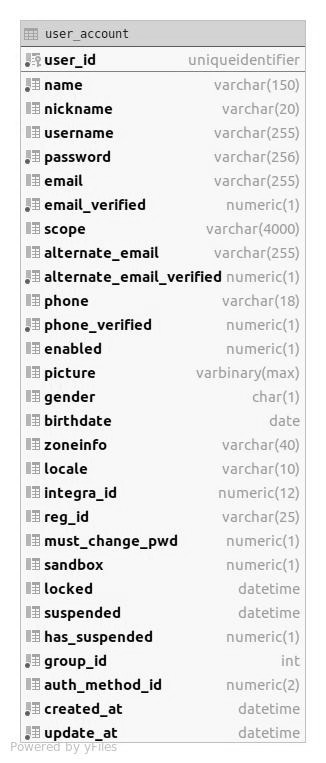
\includegraphics[width=0.5\textwidth]{bab4/figures/tabel_user_account.jpg}
    \caption{Tabel User (user\_account)}
    \label{tabel_user_account}
\end{figure}

\subsection{Implementasi Tabel Group}
\par Tabel group digunakan untuk menyimpan data kelompok pengguna. Kode yang digunakan untuk membuat tabel dapat dilihat pada Kode Sumber \ref{code:pn_group} dan hasil tabel dapat dilihat pada Gambar \ref{tabel_pn_group}.
\lstinputlisting[label=code:pn_group, caption=Implementasi Tabel Group, language=SQL]{bab4/sql/pn_group.sql}
\begin{figure}[H]
    \centering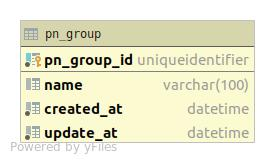
\includegraphics[width=0.5\textwidth]{bab4/figures/tabel_pn_group.jpg}
    \caption{Tabel Group (pn\_group)}
    \label{tabel_pn_group}
\end{figure}

\subsection{Implementasi Tabel Group Member}
\par Tabel group member digunakan untuk menyimpan data anggota kelompok pengguna. Kode yang digunakan untuk membuat tabel dapat dilihat pada Kode Sumber \ref{code:pn_group_member} dan hasil tabel dapat dilihat pada Gambar \ref{tabel_pn_group_member}.
\lstinputlisting[label=code:pn_group_member, caption=Implementasi Tabel Group Member, language=SQL]{bab4/sql/pn_group_member.sql}
\begin{figure}[H]
    \centering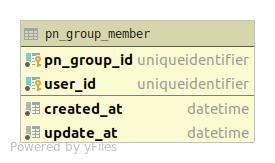
\includegraphics[width=0.5\textwidth]{bab4/figures/tabel_pn_group_member.jpg}
    \caption{Tabel Group Member (pn\_group\_member)}
    \label{tabel_pn_group_member}
\end{figure}

\subsection{Implementasi Tabel Client}
\par Tabel client digunakan untuk menyimpan data aplikasi. Kode yang digunakan untuk membuat tabel dapat dilihat pada Kode Sumber \ref{code:oauth_client} dan hasil tabel dapat dilihat pada Gambar \ref{tabel_oauth_client}.
\lstinputlisting[label=code:oauth_client, caption=Implementasi Tabel Client, language=SQL]{bab4/sql/oauth_client.sql}
\begin{figure}[H]
    \centering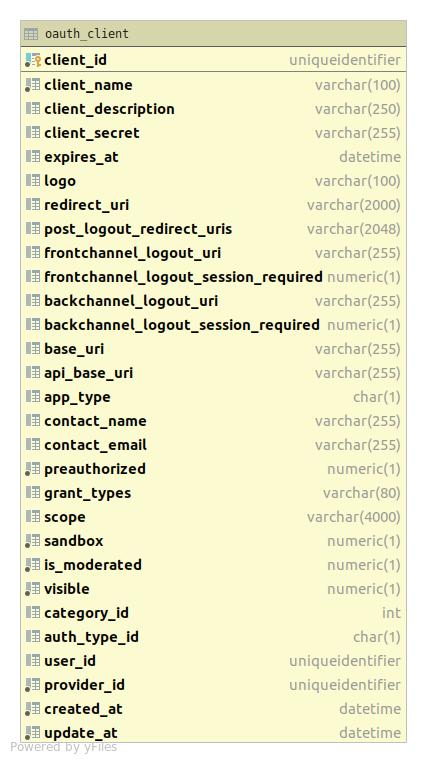
\includegraphics[width=0.5\textwidth]{bab4/figures/tabel_oauth_client.jpg}
    \caption{Tabel Client (oauth\_client)}
    \label{tabel_oauth_client}
\end{figure}

\subsection{Implementasi Tabel Certificate}
\par Tabel certificate digunakan untuk menyimpan data sertifikat client untuk autentikasi ke layanan APNs dan FCM. Kode yang digunakan untuk membuat tabel dapat dilihat pada Kode Sumber \ref{code:pn_certificate} dan hasil tabel dapat dilihat pada Gambar \ref{tabel_pn_certificate}.
\lstinputlisting[label=code:pn_certificate, caption=Implementasi Tabel Certificate, language=SQL]{bab4/sql/pn_certificate.sql}
\begin{figure}[H]
    \centering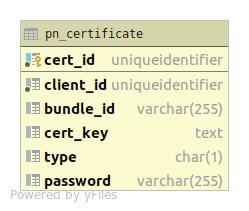
\includegraphics[width=0.5\textwidth]{bab4/figures/tabel_pn_certificate.jpg}
    \caption{Tabel Certificate (pn\_certificate)}
    \label{tabel_pn_certificate}
\end{figure}

\subsection{Implementasi Tabel Device}
\par Tabel device digunakan untuk menyimpan data perangkat pengguna yang terdaftar di layanan APNs dan FCM. Kode yang digunakan untuk membuat tabel dapat dilihat pada Kode Sumber \ref{code:device_token} dan hasil tabel dapat dilihat pada Gambar \ref{tabel_device_token}.
\lstinputlisting[label=code:device_token, caption=Implementasi Tabel Device, language=SQL]{bab4/sql/device_token.sql}
\begin{figure}[H]
    \centering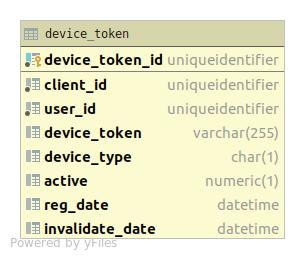
\includegraphics[width=0.5\textwidth]{bab4/figures/tabel_device_token.jpg}
    \caption{Tabel Device (device\_token)}
    \label{tabel_device_token}
\end{figure}

\subsection{Implementasi Tabel Batch}
\par Tabel batch digunakan untuk menyimpan data notifikasi yang akan dikirim ke beberapa pengguna atau kelompok. Kode yang digunakan untuk membuat tabel dapat dilihat pada Kode Sumber \ref{code:pn_batch} dan hasil tabel dapat dilihat pada Gambar \ref{tabel_pn_batch}.
\lstinputlisting[label=code:pn_batch, caption=Implementasi Tabel Batch, language=SQL]{bab4/sql/pn_batch.sql}
\begin{figure}[H]
    \centering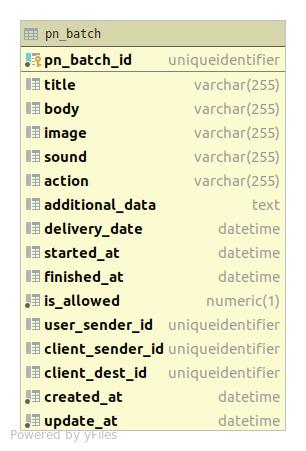
\includegraphics[width=0.5\textwidth]{bab4/figures/tabel_pn_batch.jpg}
    \caption{Tabel Batch (pn\_batch)}
    \label{tabel_pn_batch}
\end{figure}

\subsection{Implementasi Tabel Packet}
\par Tabel packet digunakan untuk menyimpan data notifikasi yang akan dikirim ke satu perangkat. Kode yang digunakan untuk membuat tabel dapat dilihat pada Kode Sumber \ref{code:pn_packet} dan hasil tabel dapat dilihat pada Gambar \ref{tabel_pn_packet}.
\lstinputlisting[label=code:pn_packet, caption=Implementasi Tabel Packet, language=SQL]{bab4/sql/pn_packet.sql}
\begin{figure}[H]
    \centering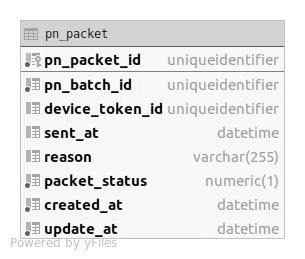
\includegraphics[width=0.5\textwidth]{bab4/figures/tabel_pn_packet.jpg}
    \caption{Tabel Packet (pn\_packet)}
    \label{tabel_pn_packet}
\end{figure}

\subsection{Implementasi Tabel User Destination}
\par Tabel user destination digunakan untuk menyimpan data pengguna yang akan menerima notifikasi dari suatu batch. Kode yang digunakan untuk membuat tabel dapat dilihat pada Kode Sumber \ref{code:pn_user_destination} dan hasil tabel dapat dilihat pada Gambar \ref{tabel_pn_user_destination}.
\lstinputlisting[label=code:pn_user_destination, caption=Implementasi Tabel User Destination, language=SQL]{bab4/sql/pn_user_destination.sql}
\begin{figure}[H]
    \centering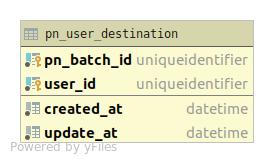
\includegraphics[width=0.5\textwidth]{bab4/figures/tabel_pn_user_destination.jpg}
    \caption{Tabel User Destination (pn\_user\_destination)}
    \label{tabel_pn_user_destination}
\end{figure}

\subsection{Implementasi Tabel Group Destination}
\par Tabel group destination digunakan untuk menyimpan data kelompok yang akan menerima notifikasi dari suatu batch. Kode yang digunakan untuk membuat tabel dapat dilihat pada Kode Sumber \ref{code:pn_group_destination} dan hasil tabel dapat dilihat pada Gambar \ref{tabel_pn_group_destination}.
\lstinputlisting[label=code:pn_group_destination, caption=Implementasi Tabel Group Destination, language=SQL]{bab4/sql/pn_group_destination.sql}
\begin{figure}[H]
    \centering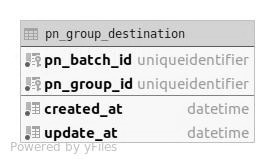
\includegraphics[width=0.5\textwidth]{bab4/figures/tabel_pn_group_destination.jpg}
    \caption{Tabel Group Destination (pn\_group\_destination)}
    \label{tabel_pn_group_destination}
\end{figure}

\section{Implementasi Antrian Pesan}
\par Subbab ini membahas bagaimana mengimplementasikan antrian pesan dengan menggunakan Kafka, meliputi konfigurasi Kafka dan sistem lain yang dibutuhkan oleh Kafka.

\subsection{Implementasi Zookeeper}
\par Zookeeper dijalankan sebagai Docker Container dengan konfigurasi yang diatur oleh Docker Compose. Zookeeper dibutuhkan oleh Kafka untuk mengatur distribusi topik, consumer, dan sebagainya. Untuk keamanan, Zookeeper dilindungi dengan metode autentikasi SASL/Digest-MD5. Hasil implementasi dapat dilihat pada Kode Sumber \ref{yaml:zookeeper}.
\lstinputlisting[label=yaml:zookeeper, caption=Konfigurasi Docker Compose untuk Zookeeper] {bab4/yaml/zookeeper.yml}

\subsection{Implementasi Kafka}
\par Kafka akan berjalan sebagai Docker Container dengan konfigurasi yang diatur oleh Docker Compose. Untuk meningkatkan performa, partisi topik ditambah menjadi 4 dan jumlah \textit{thread} jaringan ditambah menjadi 16. Untuk keamanan, Kafka dilindungi dengan metode autentikasi SASL/PLAINTEXT. Hasil implementasi dapat dilihat pada Kode Sumber \ref{yaml:kafka}.
\lstinputlisting[label=yaml:kafka, caption=Konfigurasi Docker Compose untuk Kafka] {bab4/yaml/kafka.yml}

\section{Implementasi Proses dan Kasus Penggunaan}
\par Subbab ini membahas implementasi proses yang dibuat berdasarkan hasil analisa dan rancangan yang telah dilakukan.

\subsection{Implementasi Pembuatan Packet}
\par Proses pembuatan \textit{packet} dilakukan secara berkala oleh modul Scheduler setiap 30 detik. \textit{Packet} yang telah dibuat akan disimpan di sistem basis data. Hasil implementasi dapat dilihat pada Kode Sumber \ref{code:pembuatan_packet}.
\lstinputlisting[label=code:pembuatan_packet, caption=Implementasi Java untuk Pembuatan Packet, language=Java] {bab4/java/pembuatan_packet.java}

\subsection{Implementasi Menambahkan Packet ke Antrian}
\par Proses menambahkan \textit{packet} ke antrian dilakukan secara berkala oleh modul Scheduler setiap 30 detik dengan jeda awal 15 detik. Tujuan penambahan jeda awal adalah untuk mengoptimalkan penggunaan sumber daya \textit{server} dengan mencegah proses pembuatan dan mengantrikan packet berjalan bersamaan. \textit{Packet} yang siap dikirim akan diantrikan ke Kafka. Hasil implementasi dapat dilihat pada Kode Sumber \ref{code:menambahkan_packet_ke_antrian}.
\lstinputlisting[label=code:menambahkan_packet_ke_antrian, caption=Implementasi Java untuk Menambahkan Packet ke Antrian, language=Java] {bab4/java/menambahkan_packet_ke_antrian.java}

\subsection{Implementasi Pengiriman Packet ke APNs}
\par Proses pengiriman \textit{packet} ke APNs dilakukan secara berkala oleh Sender APN dengan cara menunggu Kafka untuk memberikan \textit{packet} yang berada diantrian topik "ios". Hasil implementasi dapat dilihat pada Kode Sumber \ref{code:pengiriman_packet_ke_apns}.
\lstinputlisting[label=code:pengiriman_packet_ke_apns, caption=Implementasi Java untuk Pengiriman Packet ke APNs, language=Java] {bab4/java/pengiriman_packet_ke_apns.java}

\subsection{Implementasi Pengiriman Packet ke FCM}
\par Proses pengiriman packet dilakukan secara berkala oleh Sender FCM dengan cara menunggu Kafka untuk mengirimkan data packet yang berada diantrian topik "android" dan "web". Hasil implementasi dapat dilihat pada Kode Sumber \ref{code:pengiriman_packet_ke_fcm}.
\lstinputlisting[label=code:pengiriman_packet_ke_fcm, caption=Implementasi Java untuk Pengiriman Packet ke FCM, language=Java] {bab4/java/pengiriman_packet_ke_fcm.java}

\subsection{Implementasi Pemantauan Aplikasi}
\par Proses pemantauan aplikasi (menampilkan penggunaan sumber daya, menampilkan status kesehatan, menampilkan konfigurasi, menampilkan log) diimplementasikan dengan menggunakan library Actuator yang sudah terintegrasi dengan kerangka kerja Spring. Untuk keamanan, API Actuator dilindungi dengan metode autentikasi HTTP Basic. Setiap modul aplikasi (Scheduler, Sender APN, dan Sender FCM) menggunakan konfigurasi Actuator yang sama. Hasil implementasi konfigurasi dan API endpoint dapat dilihat pada Kode Sumber \ref{yaml:actuator} dan Tabel \ref{t:api_actuator}.
\lstinputlisting[label=yaml:actuator, caption=Konfigurasi Actuator] {bab4/yaml/actuator.yml}

\begin{longtable}{|p{3cm}|p{4.5cm}|p{1.5cm}|}
	\caption{API Endpoint Actuator} \label{t:api_actuator} \\ \hline
	\textbf{API Endpoint} & \textbf{Deskripsi} & \textbf{Format} \\ \hline
	/actuator/metrics & Menampilkan daftar metrik penggunaan sumber daya & JSON \\ \hline
	/actuator/metrics/* & Menampilkan rincian metrik penggunaan sumber daya & JSON \\ \hline
	/actuator/health & Menampilkan daftar kondisi kesehatan layanan yang terhubung & JSON \\ \hline
	/actuator/env & Menampilkan konfigurasi lingkungan & JSON \\ \hline
	/actuator/logfile & Menampilkan isi \textit{log} & Text \\ \hline
\end{longtable}
